\paragraph{QuizziPedia::Front-End::Controllers::QuestionsController}
\begin{figure} [ht]
	\centering
	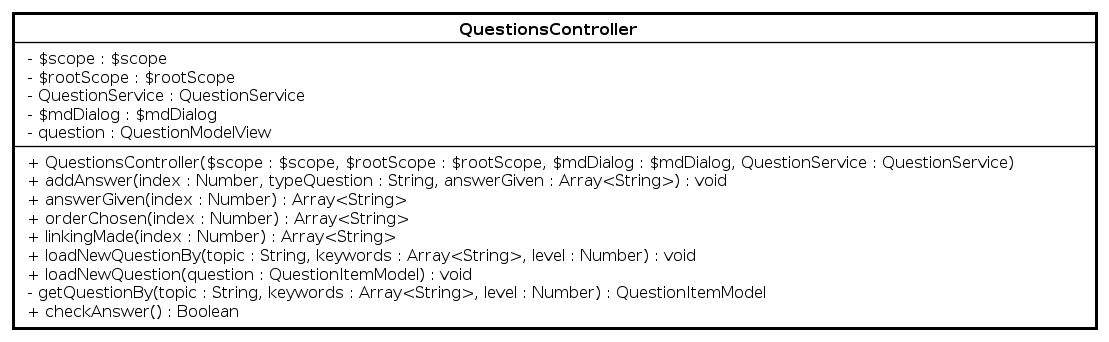
\includegraphics[scale=0.25]{UML/Classi/Front-End/QuizziPedia_Front-end_Controller_QuestionsController.png}
	\caption{QuizziPedia::Front-End::Controllers::QuestionsController}
\end{figure} \FloatBarrier
\begin{itemize}
	\item \textbf{Descrizione}: questa classe permette di gestire il recupero delle domande per far si che possano essere visualizzate nella modalità allenamento e nella compilazione dei questionari;
	\item \textbf{Utilizzo}: fornisce le funzionalità per il recupero delle domande esistenti nel database al fine di poterle visualizzare nella modalità allenamento e nella compilazione dei questionari;
	\item \textbf{Relazione con altre classi}:
	\begin{itemize}
		\item \textbf{IN \texttt{QuestionsModelView}}: classe di tipo \textit{modelview\ped{G}} la cui istanziazione è contenuta all'interno della variabile di ambiente \$scope di \textit{Angular\ped{G}}. All'interno di essa sono presenti le variabili e i metodi necessari per il \textit{Two-Way Data-Binding\ped{G}} tra le \textit{directive\ped{G}} che compongono dinamicamente la vista della domanda e il \textit{controller\ped{G}} \texttt{QuestionsController};
		\item \textbf{IN \texttt{QuestionServices}}: questa classe permette di ottenere domande esistenti e salvare nuove domande;
		\item \textbf{IN \texttt{QuestionItemModel}}: rappresenta una domanda. Contiene tutte le informazioni necessarie alla presentazione del contenuto della domanda;
		\item \textbf{OUT \texttt{FillingQuestionnaireController}}: questa classe permette di gestire la compilazione del questionario;
		\item \textbf{OUT \texttt{TrainingController}}: questa classe permette di gestire la modalità allenamento sottoponendo all'utente le giuste domande adatte al suo livello.
	\end{itemize}
	\item \textbf{Attributi}:
	\begin{itemize}
		\item \texttt{-} \texttt{\$scope: \$scope} \\
		Campo dati contenente un riferimento all'oggetto \$scope creato da \textit{Angular\ped{G}}, viene utilizzato come mezzo di comunicazione tra il \textit{controller\ped{G}} e la \textit{view\ped{G}}. Contiene gli oggetti che definiscono il \textit{model\ped{G}} dell'applicazione;
		\item \texttt{-} \texttt{\$rootScope: \$rootScope} \\
		Campo dati contenente il riferimento all'oggetto globale \$rootScope creato da \textit{Angular\ped{G}}. Viene utilizzato per rendere accessibile a tutti i \textit{controller\ped{G}} e a tutte le \textit{view\ped{G}} l'oggetto \texttt{QuestionItemModel}. In questo caso viene utilizzato per inserire in \$rootScope l'oggetto di ritorno della chiamata a \texttt{getQuestion} del \textit{service\ped{G}} \texttt{QuestionsService};
		\item \texttt{-} \texttt{\$mdDialog: \$mdDialog} \\
		Campo dati contenente un riferimento al servizio della libreria \textit{Material for Angular\ped{G}} che permette di creare delle componenti a pop-up;
		\item \texttt{-} \texttt{QuestionService: QuestionsService}\\ Permette di ottenere domande esistenti tramite chiamata di metodo specifici;
		\item \texttt{-} \texttt{question: QuestionsModelView} \\
		Classe di tipo \textit{modelview\ped{G}} la cui istanziazione è contenuta all'interno della variabile di ambiente \$scope di \textit{Angular\ped{G}}. All'interno di essa sono presenti le variabili e i metodi necessari per il \textit{Two-Way Data-Binding\ped{G}} tra le \textit{directive\ped{G}} che compongono dinamicamente la vista della domanda e il \textit{controller\ped{G}} \texttt{QuestionsController}.
	\end{itemize}
	\item \textbf{Metodi}:
	\begin{itemize}
		\item \texttt{+} \texttt{QuestionsController(\$scope: \$scope, \$rootScope: \$rootScope, \$mdDia-\\log: \$mdDialog, QuestionService: QuestionService, \$timeout: \$timeout, \$location: \$location, \$routeParams, ErrorInfoModel: ErrorInfoModel, QuestionItemModel: QuestionItemModel, Utils: Utils)} \\ Metodo costruttore della classe. Interagendo con l'oggetto \texttt{QuestionItemModel} ricevuto si interfaccia con la \textit{view\ped{G}} andando a visualizzare la giusta \textit{directive\ped{G}} della tipologia di domanda. \\
		\textbf{Parametri}:
		\begin{itemize}
			\item \texttt{\$scope: \$scope} \\
			Campo dati contenente un riferimento all'oggetto \$scope creato da \textit{Angular\ped{G}}. Viene utilizzato come mezzo di comunicazione tra il \textit{controller\ped{G}} e la \textit{view\ped{G}}. Contiene gli oggetti che definiscono il \textit{viewmodel\ped{G}} e il \textit{model\ped{G}} dell'applicazione;
			\item \texttt{\$rootScope: \$rootScope} \\
			Parametro contenente il riferimento all'oggetto globale \$rootScope creato da \textit{Ang-\\ular\ped{G}}. Viene utilizzato per rendere accessibile a tutti i \textit{controller\ped{G}} e a tutte le \textit{view\ped{G}} l'oggetto \texttt{QuestionItemModel}. In questo caso viene utilizzato per inserire in \$rootScope l'oggetto di ritorno della chiamata a \texttt{getQuestion} del \textit{service\ped{G}} \texttt{QuestionsServ-\\ice}; 
			\item \texttt{\$mdDialog: \$mdDialog} \\
			Parametro contenente un riferimento al servizio della libreria \textit{Material for Angular\ped{G}} che permette di creare delle componenti a pop-up;
			\item \texttt{QuestionService: QuestionService} \\ Parametro che permette di ottenere domande esistenti tramite chiamata di metodo specifici;
			\item \timeoutP;
			\item \locationP;
			\item \routeparamsP;
			\item \errorinfomodelP;
			\item \questionitemmodelP;
			\item \utilsP.
		\end{itemize}
		\item \texttt{+} \texttt{addAnswer(index: Number, typeQuestion: String, answerGiven: \\Array<String>): void} \\
		Metodo che gestisce l'evento di selezione delle risposte. \\
		\textbf{Parametri}:
		\begin{itemize}
			\item \texttt{index: Number} \\
			Parametro contenente l'indice della risposta di cui si vuole tenere traccia. Rappresenta anche l'indice dell'array \texttt{answerGiven} in cui verrà inserito l'oggetto delle risposte date;
			\item \texttt{typeQuestion: String} \\
			Parametro contenente una stringa la quale indica la tipologia della domanda;
			\item \texttt{answerGiven: Array<String>} \\
			Parametro contenente l'array di risposte date dall'utente aggiornato all'ultima iterazione.
		\end{itemize}
		\item \texttt{+} \texttt{save(index: Number): Array<String>} \\
		Metodo di supporto che ritorna un array di stringhe contenente le risposte date. Si occupa di recuperare le risposte date nelle domande vero/falso, risposta multipla e ad area cliccabile.\\
		\textbf{Parametri}:
		\begin{itemize}
			\item \texttt{index: Number} \\
			Parametro contenente l'indice della risposta di cui si vuole raccogliere le risposte date. 
		\end{itemize}
		\item \texttt{-} \texttt{downloadNextQuestionTraining(nextQuestion: Object): void} \\
		Metodo che gestisce l'evento per scaricare una nuova domanda in base ai parametri passati. Evoca l'evento per inserire la domanda in \texttt{TrainingModelView}. \\
		\textbf{Parametri}:
		\begin{itemize}
			\item \texttt{nextQuestion: Object} \\
			Parametro contenente un oggetto così fatto: \\
			\textbf{Parametri}:
			\begin{itemize}
				\item \texttt{language: String} \\
				Parametro contenente la lingua della domanda;
				\item \texttt{topic: String} \\
				Parametro contenente l'argomento della domanda;
				\item \texttt{keywords: Array<String>} \\
				Parametro contenente un array di stringhe che rappresenta le keywords scelte per l'allenamento;
				\item \texttt{level: Number} \\
				Parametro contenente il livello dell'utente;
				\item \texttt{alreadyAnswered: Array<String>} \\
				Parametro contenente un array di stringhe che rappresenta le domande già risposte fino a quel momento dell'allenamento;
			\end{itemize}
		\end{itemize}
		\item \texttt{-} \texttt{loadNextQuestionQuiz(question: QuestionItemModel): void} \\
		Metodo che gestisce l'evento per visualizzare una nuova domanda. \\
		\textbf{Parametri}:
		\begin{itemize}
			\item \texttt{question: QuestionItemModel} \\
			Parametro contenente un riferimento all'oggetto di tipo \texttt{QuestionItemModel}.
		\end{itemize}
		\item \texttt{+} \texttt{checkAnswer(): Boolean} \\ 
		Metodo che controlla che le risposte date siano corrette;
		\item \texttt{+} \texttt{dragnNDropQuestions(event: Object, ui: Object, index: Number, type: String, obj: Array<String>): void} 
		Metodo che gestisce l'evento per l'inserimento delle risposte date con una domanda che ha il trascinamento come base di interazione con l'utente. \\
		\textbf{Parametri}:
		\begin{itemize}
			\item \texttt{(event: Object} \\
			Parametro necessario per catturare l'evento di trascinamento;
			\item \texttt{ui: Object} \\
			Parametro necessario per capire quale oggetto viene trascinato;
			\item \texttt{index: Number} \\
			Parametro contenente l'indice della risposta di cui si vuole tenere traccia. Rappresenta anche l'indice dell'array \texttt{answerGiven} in cui verrà inserito l'oggetto delle risposte date;
			\item \texttt{typeQuestion: String} \\
			Parametro contenente una stringa la quale indica la tipologia della domanda;
			\item \texttt{answerGiven: Array<String>} \\
			Parametro contenente l'array di risposte date dall'utente aggiornato all'ultima iterazione.
		\end{itemize}
		\item \texttt{-} \texttt{\$on('loadNewQuestion': String, callback: function): void} \\
		Metodo che gestisce l'evento per scaricare una nuova domanda. \\
		\textbf{Parametri}:
		\begin{itemize}
			\item \texttt{-} \texttt{'loadNewQuestion': String: String} \\
			Parametro che indica su quale evento rimanere in ascolto;
			\item \texttt{-} \texttt{callback: function} \\
			Parametro che indica una funzione da eseguire.
		\end{itemize}
		\item \texttt{+} \texttt{\$on('loadNewQuestionQuiz': String, callback: function): void} \\
		Metodo che gestisce l'evento per caricare una nuova domanda di un questionario.\\
		\textbf{Parametri}:
		\begin{itemize}
			\item \texttt{-} \texttt{'loadNewQuestionQuiz': String} \\
			Parametro che indica su quale evento rimanere in ascolto;
			\item \texttt{-} \texttt{callback: function} \\
			Parametro che indica una funzione da eseguire.
		\end{itemize}
		\item \texttt{+} \texttt{\$on('checkAnswerEvent': String, callback: function): void} \\
		Metodo che gestisce l'evento per lanciare la catena di operazioni per la correzione di una domanda. \\
		\textbf{Parametri}:
		\begin{itemize}
			\item \texttt{-} \texttt{'checkAnswerEvent': String} \\
			Parametro che indica su quale evento rimanere in ascolto;
			\item \texttt{-} \texttt{callback: function} \\
			Parametro che indica una funzione da eseguire.
		\end{itemize}
	\end{itemize}
\end{itemize}

